% !TeX spellcheck = pl_PL
\newpage
\section{Wdrożenie i testowanie systemu \NazwaSys} \label{sec:testy}
Rozdział skupiać się będzie na przedstawieniu działania systemu oraz w jakim środowisku zostało testowane. Wizualizacja funkcjonowania modułów, będzie jednocześnie, krótkimi testami poprawności zaprojektowanych poszczególnych części implementacji. 

\subsection{Środowisko testowe}
Stanowisko testowe podczas implementacji projektu składa się z:
\begin{itemize*}
	\item laptopa z systemem Windows 10 EDU służącego, jako serwer (aplikacja serwerowa, baza danych),
	\item mikrokomputera Raspberry Pi 3 Model B, jako urządzenie sterujące oraz moduł zliczania osób,
	\item kamera IP Dahua DH-IPC-HDW2220RP-ZS, jako kamera zliczająca,
	\item 3 smartphony różnych modeli:
	\begin{enumerate*}
		\item Samsung S5 Neo (Android 6.0),
		\item Samsung S5 (Android 6.0),
		\item ZTE Blade A452 (Android 5.1).
	\end{enumerate*}
\end{itemize*}

Testowy laptop posiada następujące parametry:
\begin{itemize*}
	\item pamięć ram 32 GB,
	\item procesor Intel Core i7-6700HQ,
	\item dysk SSD NVMe o średniej prędkości odczytu 1,6GB/s i odczycie 920MB/s,
	\item karta graficzna Nvidia Quadro M2000M,
	\item karta sieciowa Intel Dual Band Wireless-AC 8260.
\end{itemize*}

\subsection{Wizualizacja działania systemu \textsl{\NazwaSys}}
Poniżej zostaną opisane poszczególne funkcje systemu wraz z opisem interakcji pomiędzy użytkownikiem oraz systemem. Podczas wizualizacji zakładamy żę cały system został poprawnie zainstalowany. Środowisko testowe zostało dokładnie opisane w poprzednim punkcie.

\begin{enumerate*}
	\item Logowanie (strona internetowa) \newline
	Test polegał na wykonaniu logowania błędnymi danymi (Rys. \ref{rys:Strona3} oraz sprawdzenia czy pomimo braku zalogowania można było uzyskać dostęp strony historii użycia zamków. \newline
	Wnioskiem z testów jest stwierdzenie poprawności komunikowania o błędnym logowaniu. Próbując przejść na stronę główna nie będąc zalogowany, zostajemy przekierowani do strony logowania.
\begin{figure}[ht!]
		\centering
		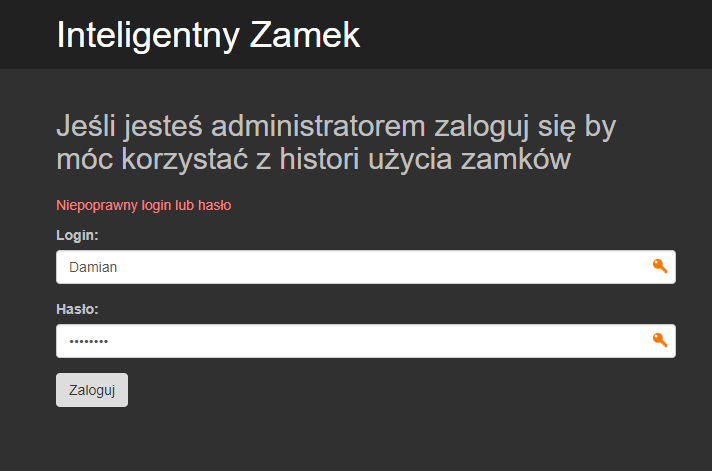
\includegraphics[width=8.5cm]{Obrazy/Strona3}
		\caption{Strona logowania -- walidacja hasła}
		\label{rys:Strona3}
\end{figure}

	\item Zliczanie osób: \newline
	 Test polegał na sprawdzeni poprawności zliczania osób w korytarzu, gdy przechodzą przez niego osoby w obie strony.
	
	Wnioski: Podczas testu wykryto prawidłową liczbę osób, które umownie ''weszły'' oraz ''wyszły''. Efekt widoczny jest na zrzutach ekranu z urządzenia sterującego. Początkowo liczniki osób wchodzących i wychodzący w lewym góry rogu ekranu wynoszą zero (Rys. \ref{rys:Kamera1}), taka sama wartość występuje przy wartości na stronie internetowej (Rys. \ref{rys:Strona1}). Rysunek \ref{rys:Kamera2} i \ref{rys:Strona2} przedstawia stan po ''wejściu'' do pomieszczenia. Działanie zliczania osób wychodzących przedstawia Rys. \ref{rys:Kamera3}.

	\begin{figure}[ht!]
		\vspace{-0.35cm}
	\begin{minipage}{0.3\textwidth}
		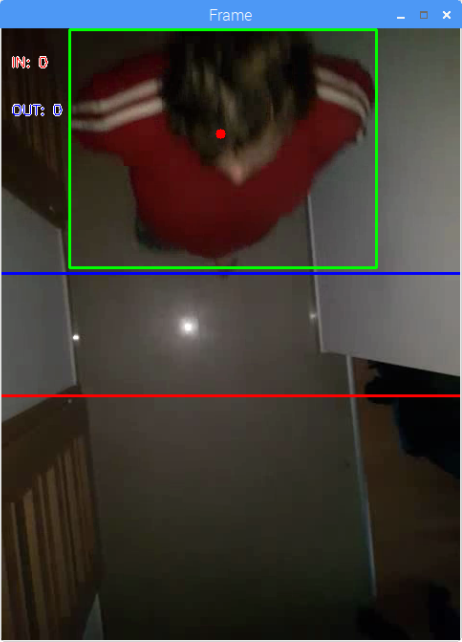
\includegraphics[width=\textwidth]{Obrazy/Kamera1}
		\caption{Stan początkowy testu zliczania osób }
		\label{rys:Kamera1}
	\end{minipage}
	\hspace{0.01\textwidth}
	\begin{minipage}{0.69\textwidth}
		\vspace{-1cm}
		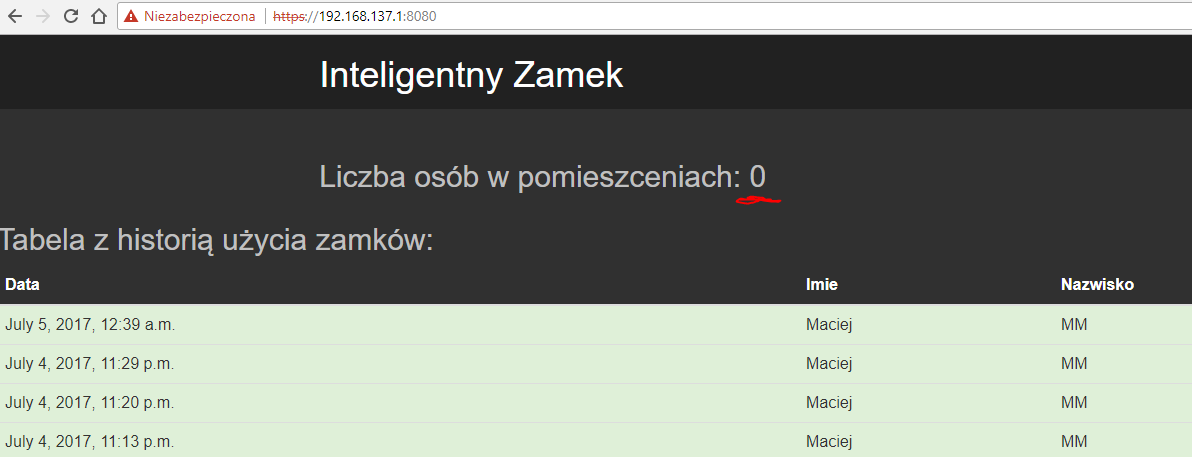
\includegraphics[width=\textwidth]{Obrazy/Strona1}
		\caption{Stan początkowy testu zliczania osób}
		\label{rys:Strona1}
	\end{minipage}
	\end{figure}

	\begin{figure}[ht!]
		\vspace{-1.5cm}
	\begin{minipage}{0.69\textwidth}
		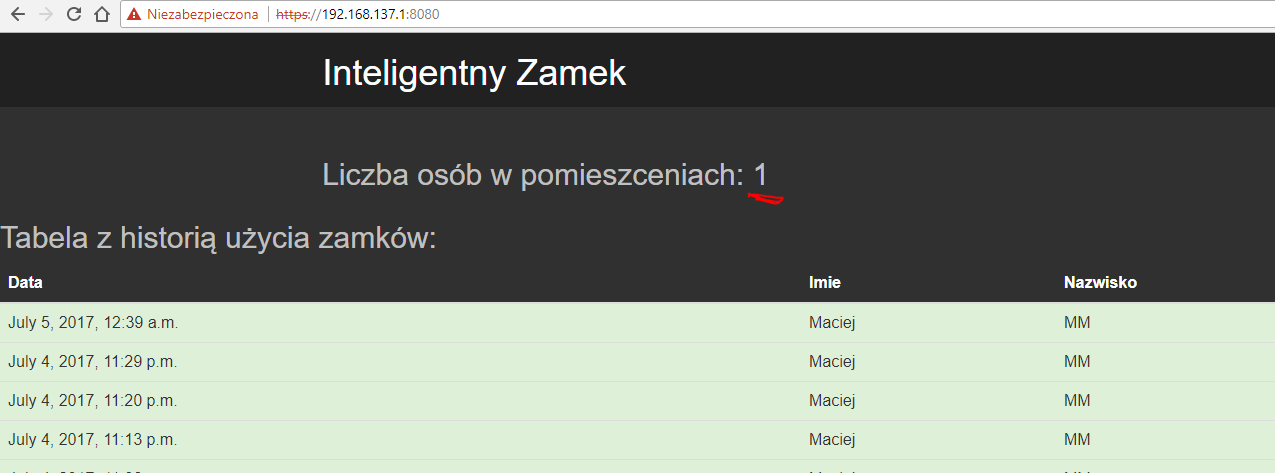
\includegraphics[width=\textwidth]{Obrazy/Strona2}
		\caption{Stan po ''wejściu'' osoby }
		\label{rys:Strona2}
	\end{minipage}
	\hspace{0.01\textwidth}
	\begin{minipage}{0.3\textwidth}
		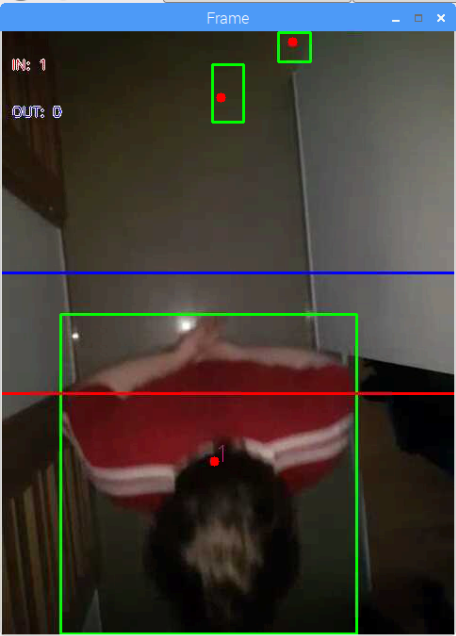
\includegraphics[width=0.9\textwidth]{Obrazy/Kamera2}
		\caption{Stan po ''wejściu'' osoby}
		\label{rys:Kamera2}
	\end{minipage}
\end{figure}

	\begin{figure}[ht!]
		\vspace{-1.7cm}
		\centering
		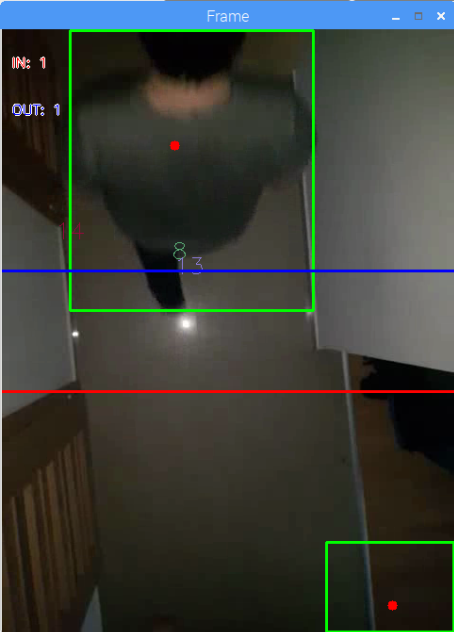
\includegraphics[width=4cm]{Obrazy/Kamera3}
		\caption{Stan po ''wyjściu'' osoby}
		\label{rys:Kamera3}
	\end{figure}
\newpage
	\item M Symulacja otwarcia
	\item M (strona) historia
	\item Logowanie użytkownika: \newline
	Test: Test polega na weryfikacji działania autoryzacji danych logowania oraz przy tym przydział odpowiednich uprawnień (administrator/zwykły użytkownik). Pierwsza próba logowania następuje z podaniem błędnego hasła użytkownika, następnie poprawnego (użytkownik TestowyZwykly) posiada zwykłe uprawnienia, trzecia próba związana będzie z zmianą uprawnień danego użytkownika na uprawnienia administratora.\newline
	Wnioski: Autoryzacja przedstawiona została na ilustracji Rys. \ref{rys:Logodwanie_blad_hasla}. Na ekranie pojawia się czerwony napis ''Błędny login lub hasło'', oznacza to w tym wypadku, że zostało podane błędne hasło (dany użytkownik istnieje w bazie danych, ale o innym haśle). Wyświetlane informacje nie wskazują na to, które dane zostały podane błędnie, przez co potencjalny włamywacz ma utrudnione zadanie przejęcia konta. Druga próba logowania skutkuje poprawnym zalogowaniem, jako użytkownik standardowy. Pojawia się okno główne, które po rozwinięciu menu wskazuje widok \ref{rys:panel_boczny_pionowo} (brak udostępnionych funkcji administracyjnych widocznych na rysunku \ref{rys:panel_boczny_pionowo2}). Trzecia próba logowania skutkuje pojawieniem się widoku \ref{rys:panel_boczny_pionowo2}, czyli zostały poprawnie przydzielone uprawnienia.
	
	\begin{figure}[ht!]
		\centering
		\includegraphics*[width=5cm]{Obrazy/APK_logowanie_blad}
		\caption{Logowanie użytkownika -- błąd hasła lub loginu}
		\label{rys:Logodwanie_blad_hasla}
	\end{figure}
	\item M rejestracja
	wyświetlanie podpowiedzi do hasła
	walidacja hasła 
	ukazywanie ukrywanie hasła
	rejestracja (komunikat +przekierowanie)
	\item M (admin)zaakceptowanie rejestracji
	widok rejestracji odrzucenie 
	akceptowanie wyniki
	\item  wnioskowanie o certyfikat\newline
	Test polegał na sprawdzeniu listy z oczekującymi certyfikatami, wykonaniu wnioskowania o certyfikat a następnie ponownym sprawdzeniu listy z oczekującymi certyfikatami.
	
	Wnioski: W stanie początkowym (Ry.s \ref{rys:wnioskowanie1}) nie było żadnego certyfikatu oczekującego na liście. Podczas wnioskowania o certyfikat w momencie wyłączenia widoku (Ry.s \ref{rys:wnioskowanie2}) wyświetlił się  komunikat o treści ''pobrano listę zamków''. W kolejnym kroku podczas naciśnięcia na pole z zamkiem (Ry.s \ref{rys:wnioskowanie3}) wyświetliła się wiadomość o treści "Wniosek został wysłany". Po ponownym sprawdzeniu na liście oczekujących certyfikatów (Ry.s \ref{rys:wnioskowanie4}) znajdował się wniosek o certyfikat. Test zakończył się pomyślnie dla tego scenariusza.
	
	
	\begin{figure}[ht!]

		\begin{minipage}{0.2\textwidth}
			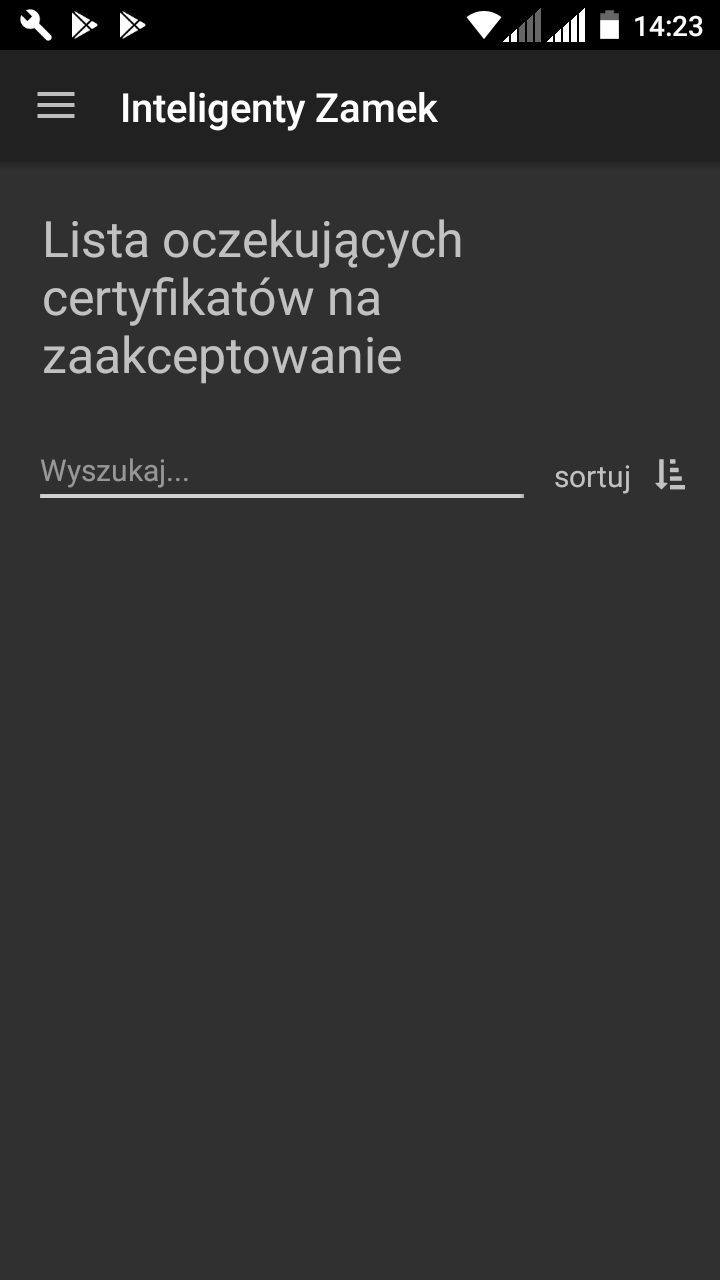
\includegraphics[width=\textwidth]{Obrazy/wnioskowanie1}
			\caption{Stan początkowy listy oczekujących certyfikatów na zaakceptowanie }
			\label{rys:wnioskowanie1}
		\end{minipage}
		\begin{minipage}{0.2\textwidth}
			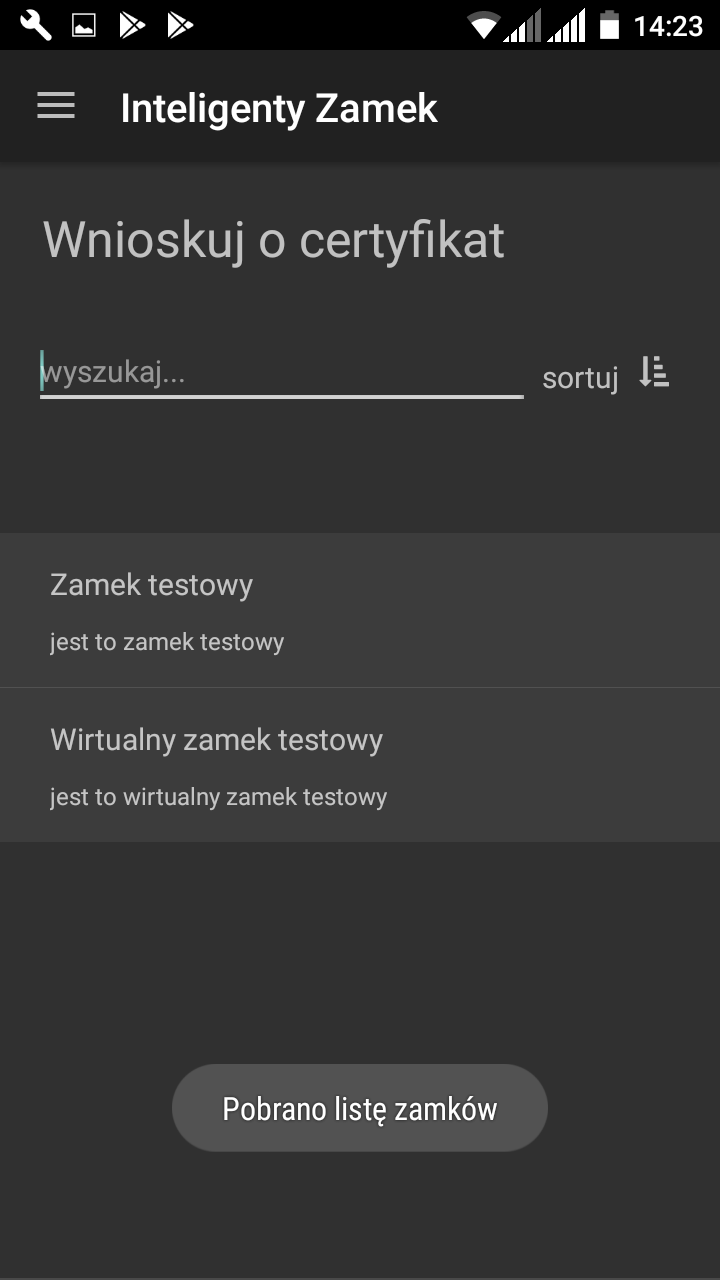
\includegraphics[width=\textwidth]{Obrazy/wnioskowanie2}
			\caption{Stan początkowy podczas załadowania widoku wnioskowania o certyfikat}
			\label{rys:wnioskowanie2}
		\end{minipage}
	
		\begin{minipage}{0.2\textwidth}
		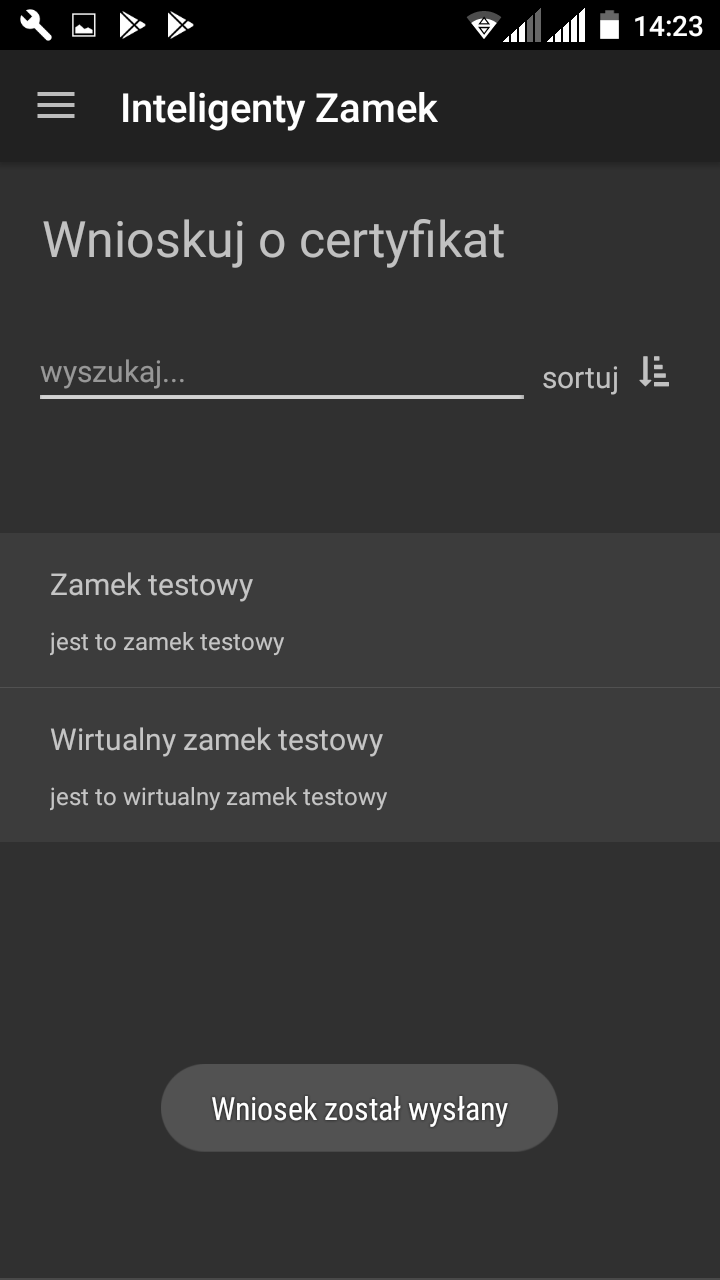
\includegraphics[width=\textwidth]{Obrazy/wnioskowanie3}
		\caption{Wnioskowanie o certyfikat}
		\label{rys:wnioskowanie3}
	\end{minipage}
	\begin{minipage}{0.2\textwidth}
		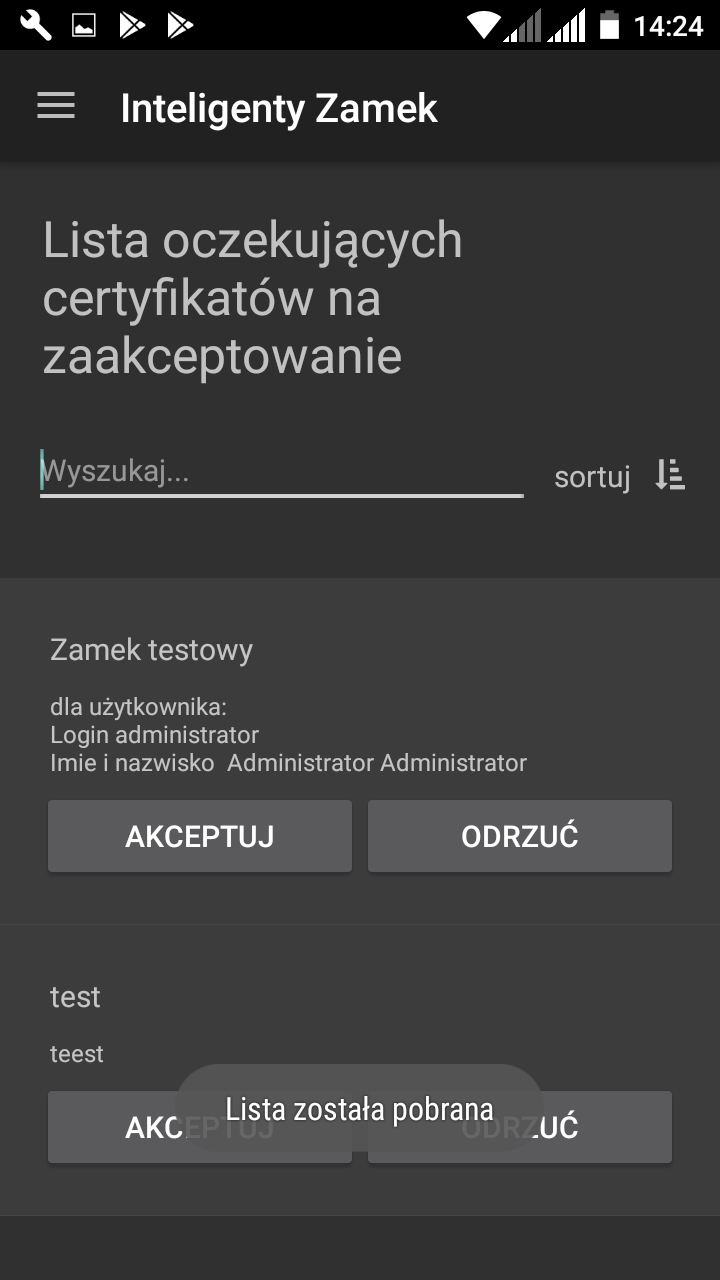
\includegraphics[width=\textwidth]{Obrazy/wnioskowanie4}
		\caption{Stan listy oczekujących certyfikatów po wnioskowaniu o certyfikat}
		\label{rys:wnioskowanie4}
	\end{minipage}
	\end{figure}
	
	
	
	
	\item wygenerowanie nowego klucza dostępowego\newline
	Test polegał na sprawdzeniu wartości certyfikatu klucza dostępowego, wygenerowaniu nowego i sprawdzenie ponowne wartości certyfikatu dostępowego.
	Wnioski: Podczas testu w stanie początkowym (Ry.s \ref{rys:generowanieKD1})znajdował się certyfikat dostępowy ważny do 2019.01.26 14:23:55. Po naciśnięciu przycisku ''Wygeneruj''  (Ry.s \ref{rys:generowanieKD2}) certyfikat został zmieniony na nowy z datą ważności o godzinę dłuższą.
 
	
	\begin{figure}[ht!]
		
		\begin{minipage}{0.4\textwidth}
			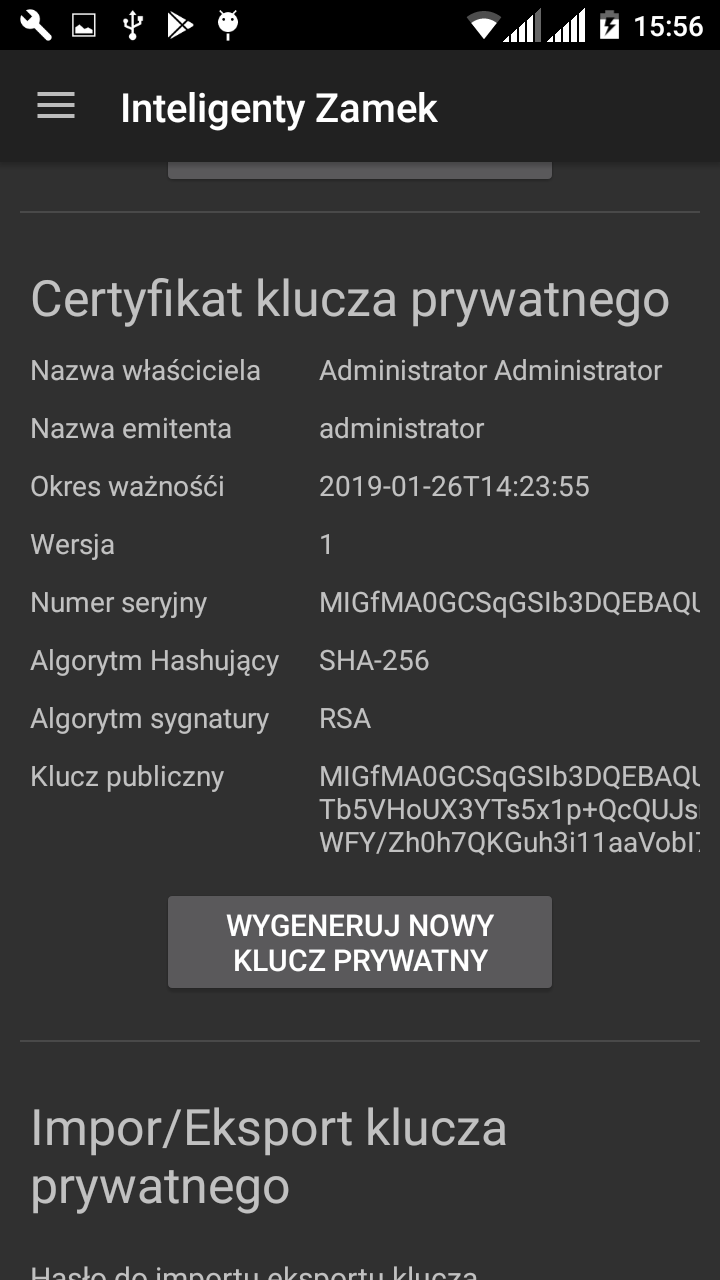
\includegraphics[width=\textwidth]{Obrazy/generowanieKD1}
			\caption{Stan początkowy wyświetlonego certyfikatu klucza dostępowego }
			\label{rys:generowanieKD1}
		\end{minipage}
		\begin{minipage}{0.4\textwidth}
			\includegraphics[width=\textwidth]{Obrazy/generowanieKD2}
			\caption{Stan po wygenerowaniu nowego certyfikatu klucza dostępowego}
			\label{rys:generowanieKD2}
		\end{minipage}
		
	
	\end{figure}
	
	
	\item  zaakceptowanie certyfikatu dostępowego przez administratora: \newline
	Test polegał na przejściu do widoku odpowiedzialnego za zarządzanie oczekującymi certyfikatami dostępu oraz odpowiednio usunięcie i zaakceptowanie wniosku.
	\newline Wnioski: w stanie początkowym znajdowały się dwa certyfikaty (Ry.s \ref{rys:generowanieCert1}. Po naciśnięciu przycisku usuń z listy zniknął dany wniosek (Ry.s \ref{rys:generowanieCert2}. Po wyborze akceptuj zostaliśmy przekierowani do widoku generowania certyfikatu. Po ponownym wejściu do listy certyfikatów (Ry.s \ref{rys:generowanieCert3}) lista ta była pusta. Test został pomyślnie przeprowadzony (Ry.s \ref{rys:generowanieCert4}). 
	
		\begin{figure}[ht!]
		
		\begin{minipage}{0.2\textwidth}
			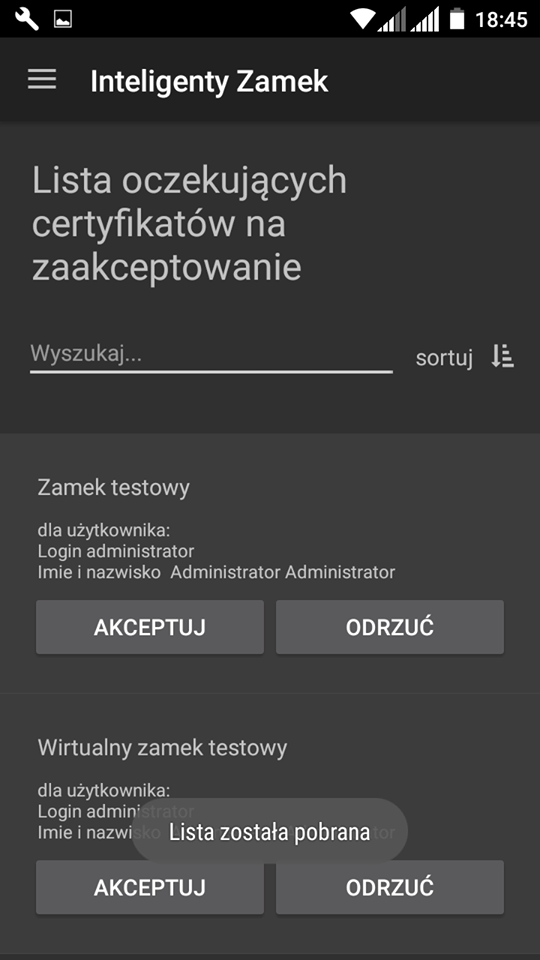
\includegraphics[width=\textwidth]{Obrazy/oczekujaceCert0}
			\caption{Stan początkowy listy oczekujących certyfikatów na zaakceptowanie }
			\label{rys:generowanieCert1}
		\end{minipage}
		\begin{minipage}{0.2\textwidth}
			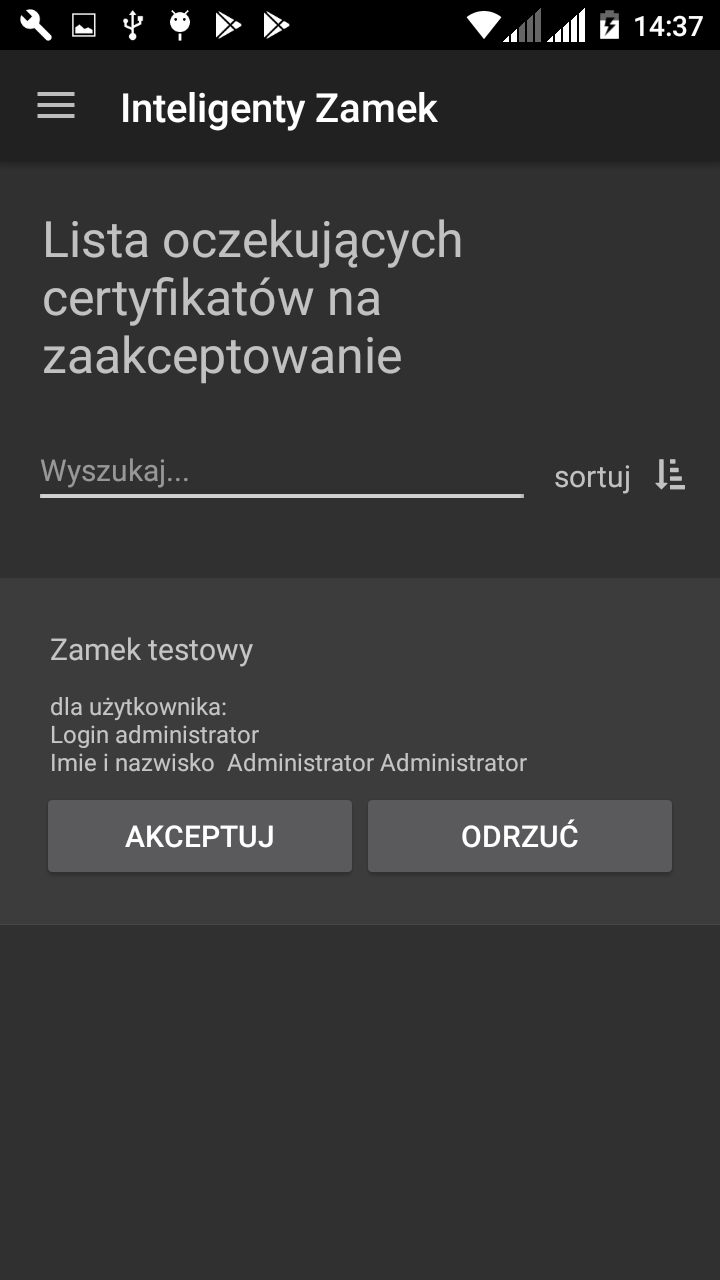
\includegraphics[width=\textwidth]{Obrazy/oczekujaceCert1}
			\caption{Stan listy oczekujących certyfikatów po usunięciu z listy elementu}
			\label{rys:generowanieCert2}
		\end{minipage}
		
		\begin{minipage}{0.2\textwidth}
			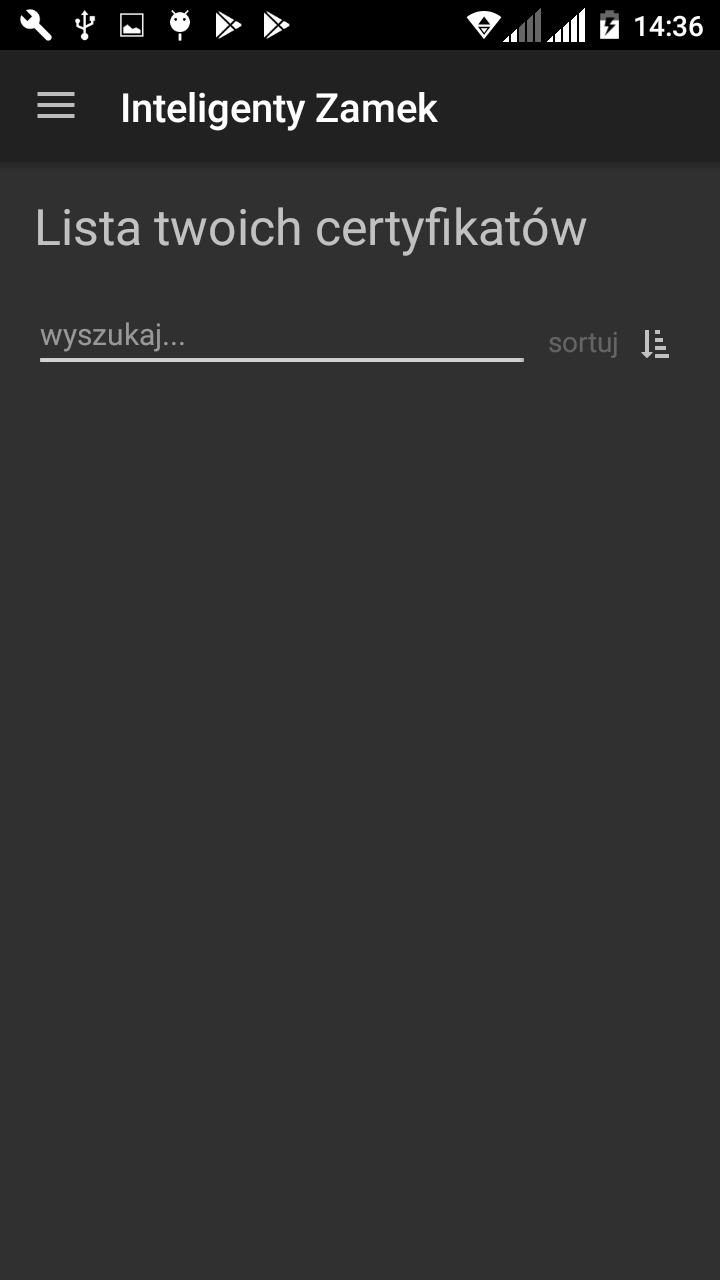
\includegraphics[width=\textwidth]{Obrazy/oczekujaceCert2}
			\caption{Stan listy oczekujących certyfikatów po ponownym otworzeniu}
			\label{rys:generowanieCert3}
		\end{minipage}
	
	\begin{minipage}{0.2\textwidth}
		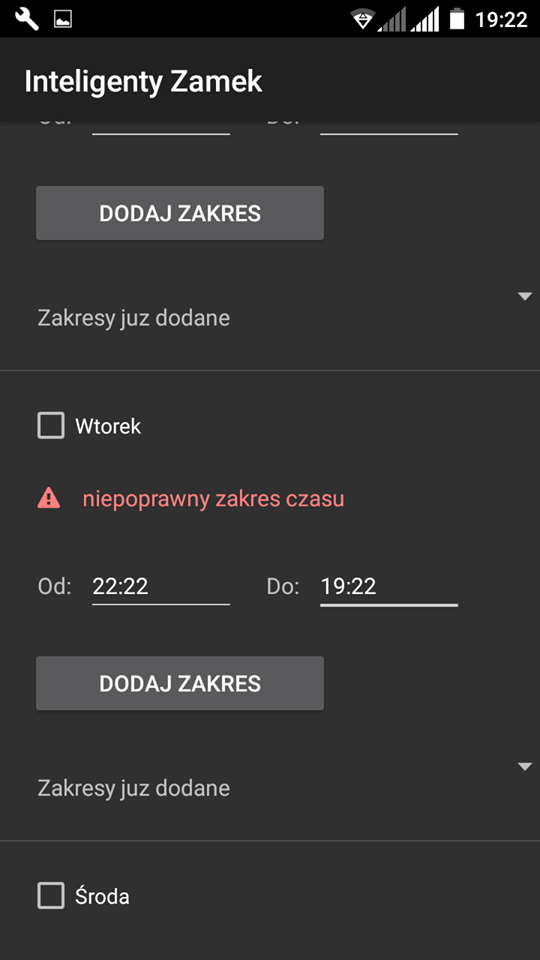
\includegraphics[width=\textwidth]{Obrazy/generowanieerror}
		\caption{Stan listy oczekujących certyfikatów po ponownym otworzeniu}
		\label{rys:generowanieCert4}
	\end{minipage}
	
	\end{figure}
	
	
	
	\item  Wygenerowanie certyfikatu dostępowego
	Test polega na przeprowadzeniu procesu generowania certyfikatu z uwzględnieniem wpisywania niepoprawnych danych.
	
	Wnioski W początkowym stanie zostały wypełnione dane użytkownika oraz wybrany został login i zamek (Ry.s \ref{rys:generowanie1}), Następnie po naciśnięciu przycisk dodaj zakresy zostało wykonane przejście do widoku  wygenerowania zakresów (Rys. \ref{rys:generowanie2}). W nim wprowadzono  błędny zakres (Rys. \ref{rys:generowanie3}). Została zwrócona walidacja (Rys. \ref{rys:generowanie4}). Następnie został dodany poprawne zakresy (Rys. \ref{rys:generowanie5}). Potem został usunięty jeden zakres (Rys. \ref{rys:generowanie6})   . Po naciśnięciu przycisku kontynuuj generowanie certyfikatu zostało wykonane przekierowanie  do dalszej części generowania certyfikatu. W widoku tym pozostały wszystkie dane uzupełnione przed przejściem do dodania zakresów. Wprowadzony został błędny zakres dat . Została wyświetlona walidacja (Rys. \ref{rys:generowanie7}).Po poprawie danych proces został pozytywnie ukończony w postaci przejścia do widoku panelu administratora.
	
	
	
		\begin{figure}[ht!]
		
		\begin{minipage}{0.2\textwidth}
			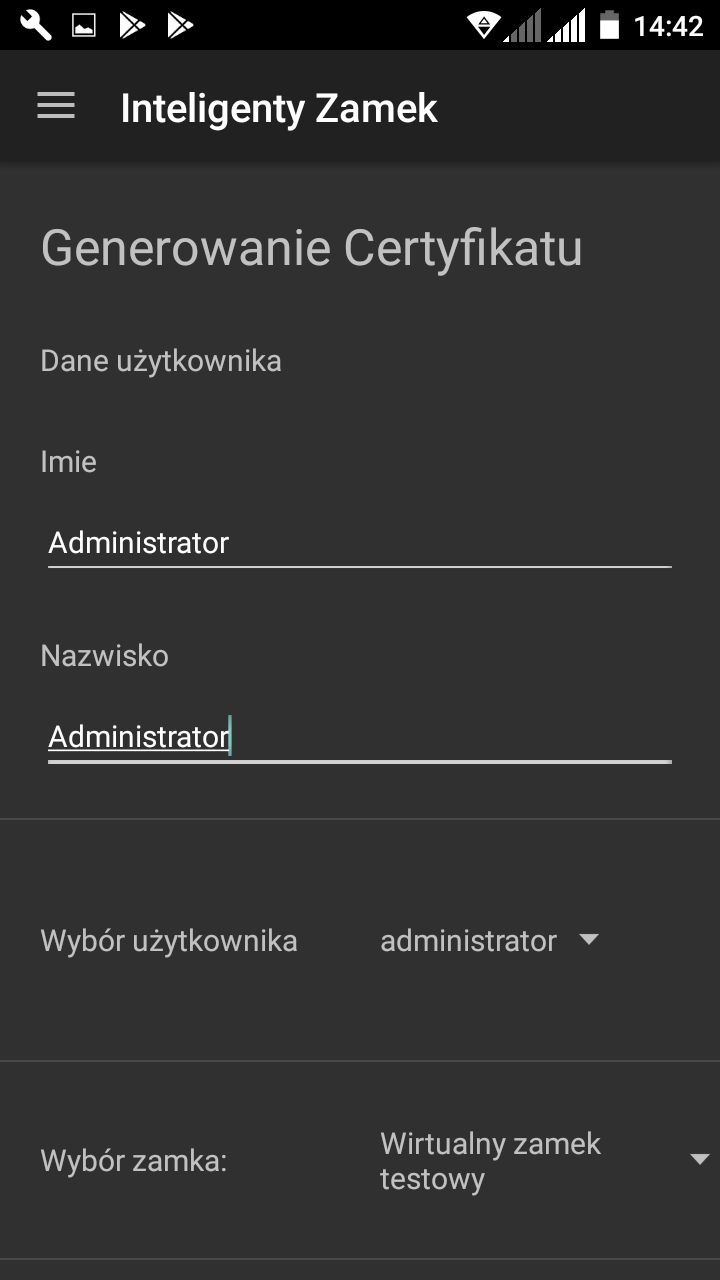
\includegraphics[width=\textwidth]{Obrazy/generowanie1}
			\caption{Stan początkowy listy oczekujących certyfikatów na zaakceptowanie }
			\label{rys:generowanie1}
		\end{minipage}
	
		
		\begin{minipage}{0.2\textwidth}
			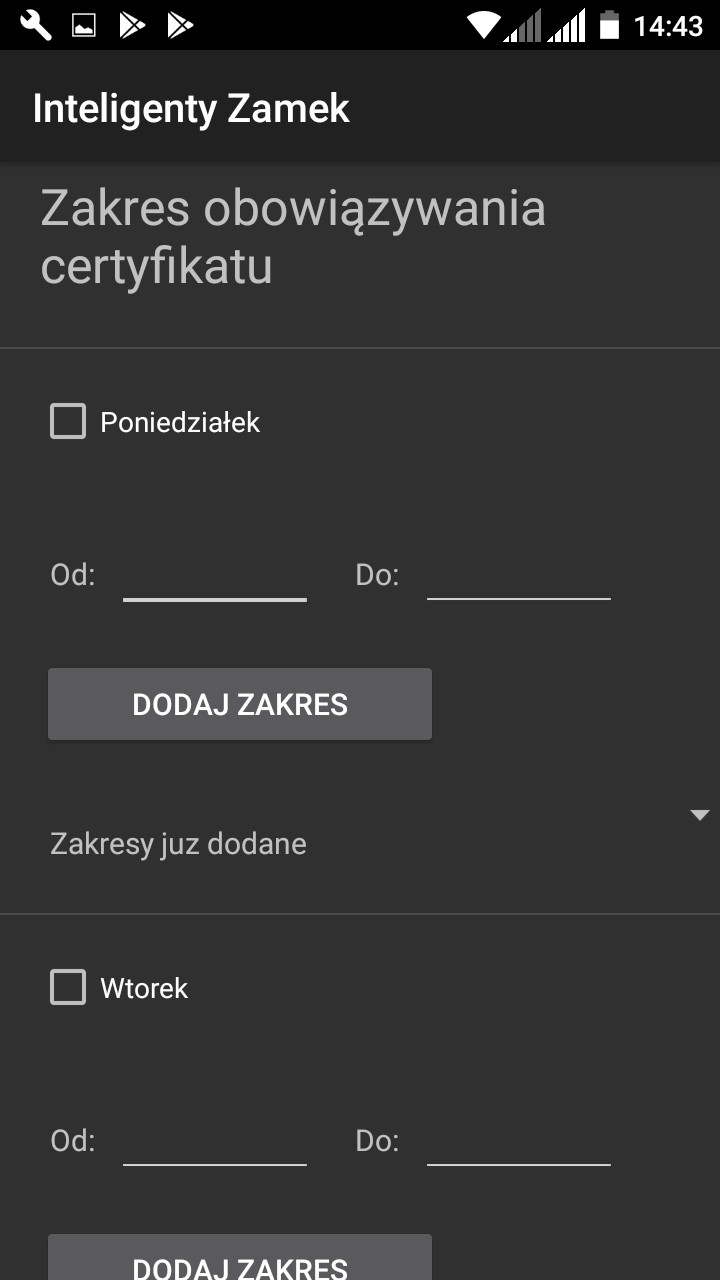
\includegraphics[width=\textwidth]{Obrazy/generowanie3}
			\caption{Wnioskowanie o certyfikat}
			\label{rys:generowanie2}
		\end{minipage}
		\begin{minipage}{0.2\textwidth}
			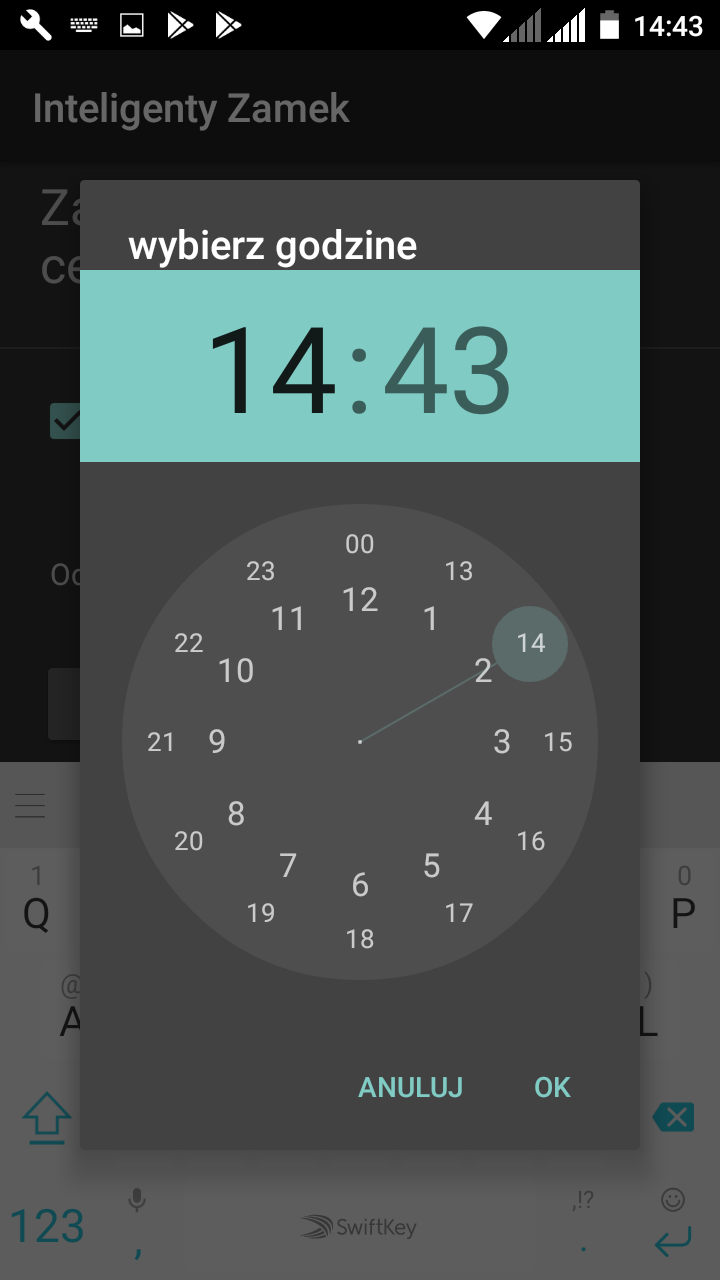
\includegraphics[width=\textwidth]{Obrazy/generowanie4}
			\caption{Stan listy oczekujących certyfikatów po wnioskowaniu o certyfikat}
			\label{rys:generowanie3}
		\end{minipage}
	\end{figure}


	


	\begin{figure}[ht!]
	
		\begin{minipage}{0.2\textwidth}
		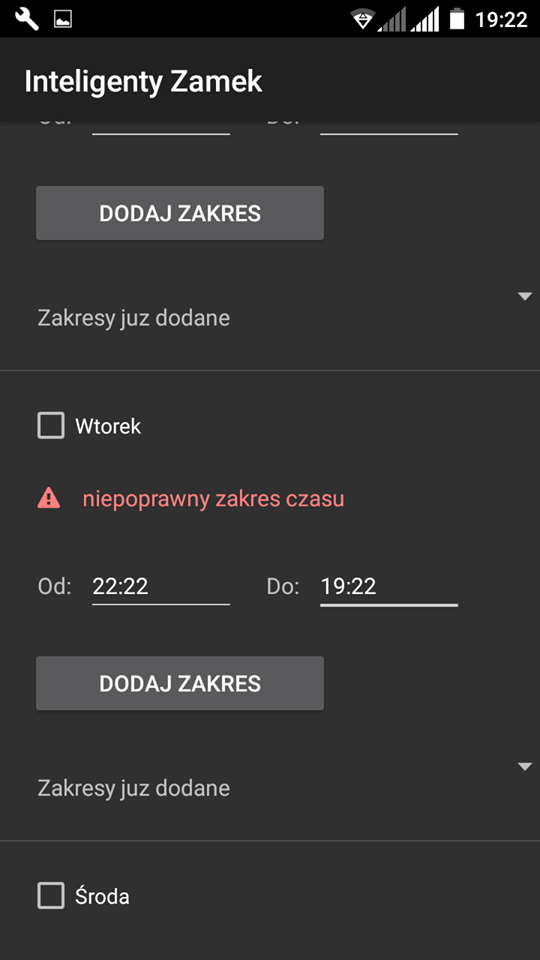
\includegraphics[width=\textwidth]{Obrazy/generowanieerror}
		\caption{Stan początkowy listy oczekujących certyfikatów na zaakceptowanie }
		\label{rys:generowanie4}
	\end{minipage}
	
		\begin{minipage}{0.2\textwidth}
		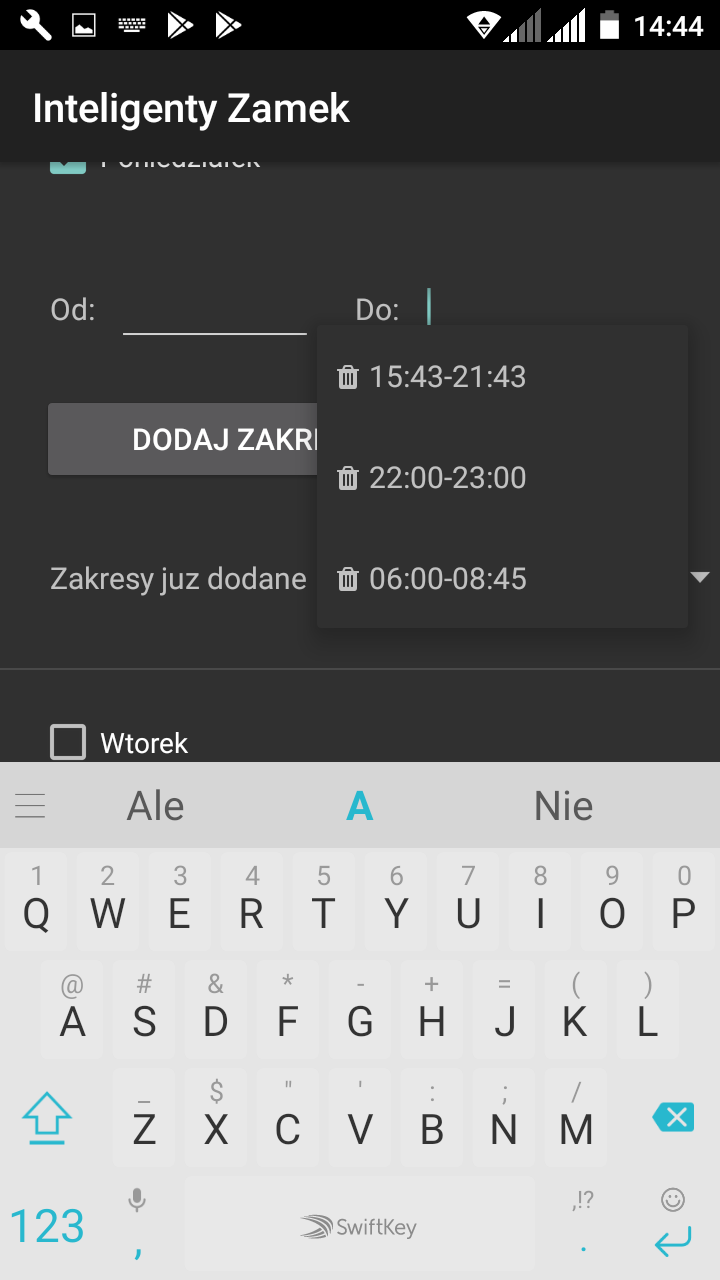
\includegraphics[width=\textwidth]{Obrazy/generowanie5}
		\caption{Stan początkowy listy oczekujących certyfikatów na zaakceptowanie }
		\label{rys:generowanie5}
	\end{minipage}
	

	\begin{minipage}{0.2\textwidth}
		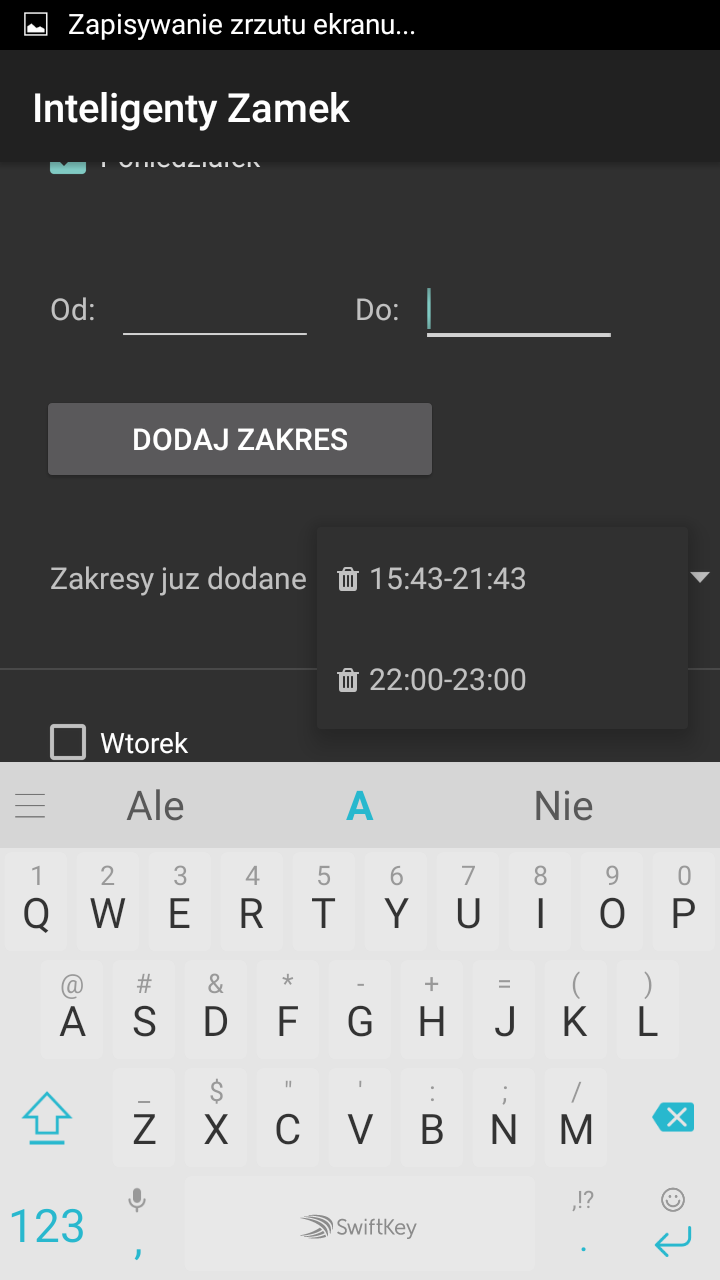
\includegraphics[width=\textwidth]{Obrazy/generowanie6}
		\caption{Stan początkowy podczas załadowania widoku wnioskowania o certyfikat}
		\label{rys:generowanie6}
	\end{minipage}
	
	\begin{minipage}{0.2\textwidth}
		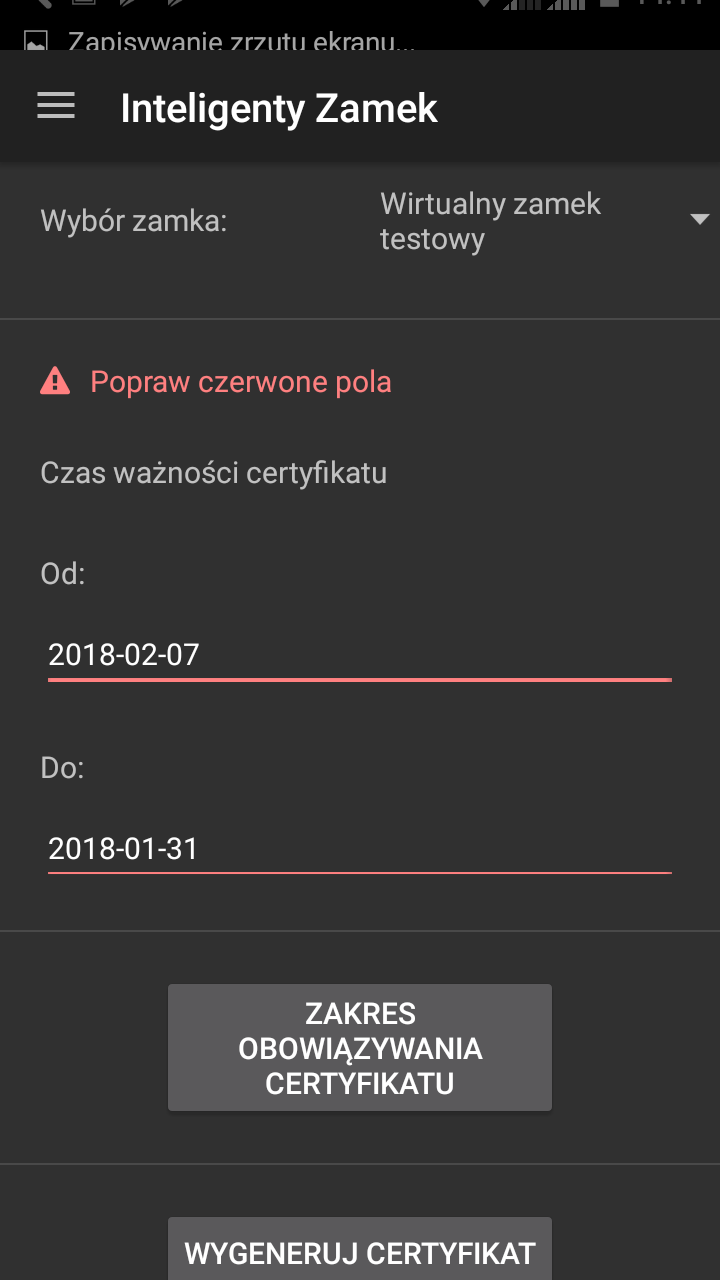
\includegraphics[width=\textwidth]{Obrazy/generowanie8}
		\caption{Wnioskowanie o certyfikat}
		\label{rys:generowanie7}
	\end{minipage}

\end{figure}
	
	
	\item   pobranie certyfikatu
	Test polegał na wyczyszczeniu pamięci telefonu. Sprawdzeniu listy certyfikatów pobraniu samych certyfikatów oraz ponownym sprawdzeniu listy certyfikatów.
	Wnioski: W stanie początkowym na liście nie były wyświetlane żadne certyfikaty (Rys. \ref{rys:getCert1}). Następnie zostało wybrane pole pobierz z serwera. W tym momencie został wyświetlony komunikat ''pobrano z serwera''(Rys. \ref{rys:getCert2}). Po ponownym przejściu do listy certyfikatów widniała już pozycja na liście (Rys. \ref{rys:getCert3}).
	
		\begin{figure}[ht!]
		
		\begin{minipage}{0.2\textwidth}
			\includegraphics[width=\textwidth]{Obrazy/getCer1}
			\caption{Stan początkowy listy oczekujących certyfikatów na zaakceptowanie }
			\label{rys:getCert1}
		\end{minipage}
		
		\begin{minipage}{0.2\textwidth}
			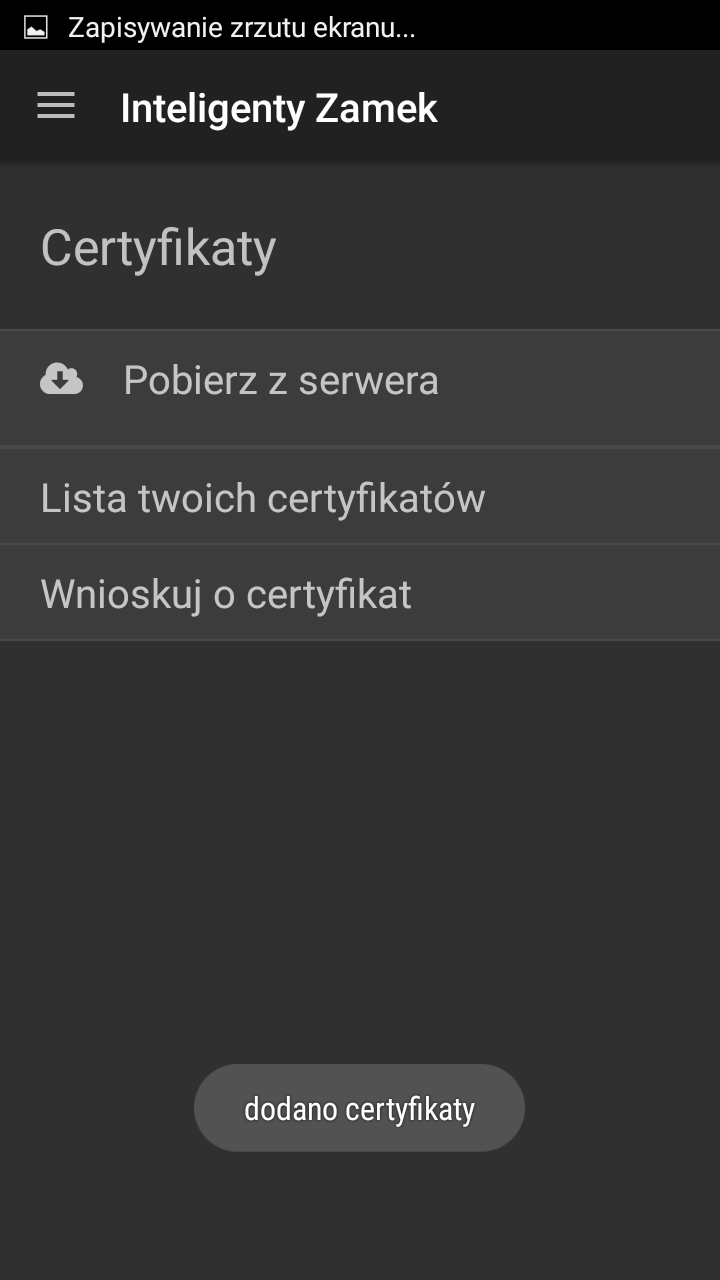
\includegraphics[width=\textwidth]{Obrazy/getCert2}
			\caption{Stan początkowy listy oczekujących certyfikatów na zaakceptowanie }
			\label{rys:getCert2}
		\end{minipage}
		
		
		\begin{minipage}{0.2\textwidth}
			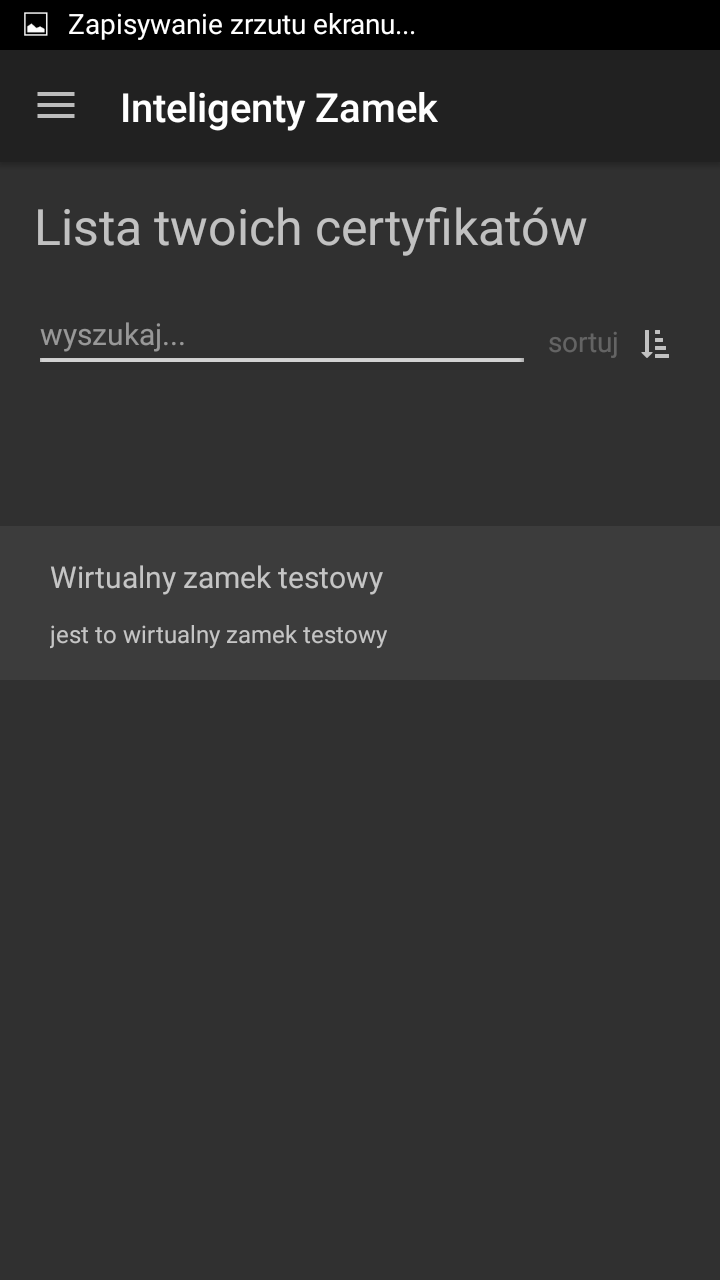
\includegraphics[width=\textwidth]{Obrazy/getCert3}
			\caption{Stan początkowy podczas załadowania widoku wnioskowania o certyfikat}
			\label{rys:getCert3}
		\end{minipage}
		
	
	\end{figure}
	
	
	\item M uzyskanie dostępu do zamka (aktywacja bluetooth)
		 jako podpunkt pokazanie braku dostępu do zamka (zmiana daty)
	\item D przedłużenie certyfikatu dostępowego
	Test polegał na naciśnięciu przycisku usuń oraz przedłuż w widoku certyfikatu (Rys. \ref{rys:przedluzCert1}).
	Wnioski dla konta administratora usuń certyfikat powodowało usunięcie go z listy i przejście do widoku certyfikatów. Przycisk przedłuż powodował przeniesienie do widoku generowania. Dla konta o uprawnieniach  mniejszych od administratora przycisk usuń działał analogicznie jak u administratora natomiast przycisk przedłuż powodował wyświetlenie komunikatu ''wysłano wniosek'' (Rys. \ref{rys:przedluzCert2}).
	Po sprawdzeniu w widoku listy oczekujących certyfikatów po wnioskowaniu, widnieje on na liście. Test został pomyślnie zakończony
	
	
		\begin{figure}[ht!]
		
		\begin{minipage}{0.2\textwidth}
			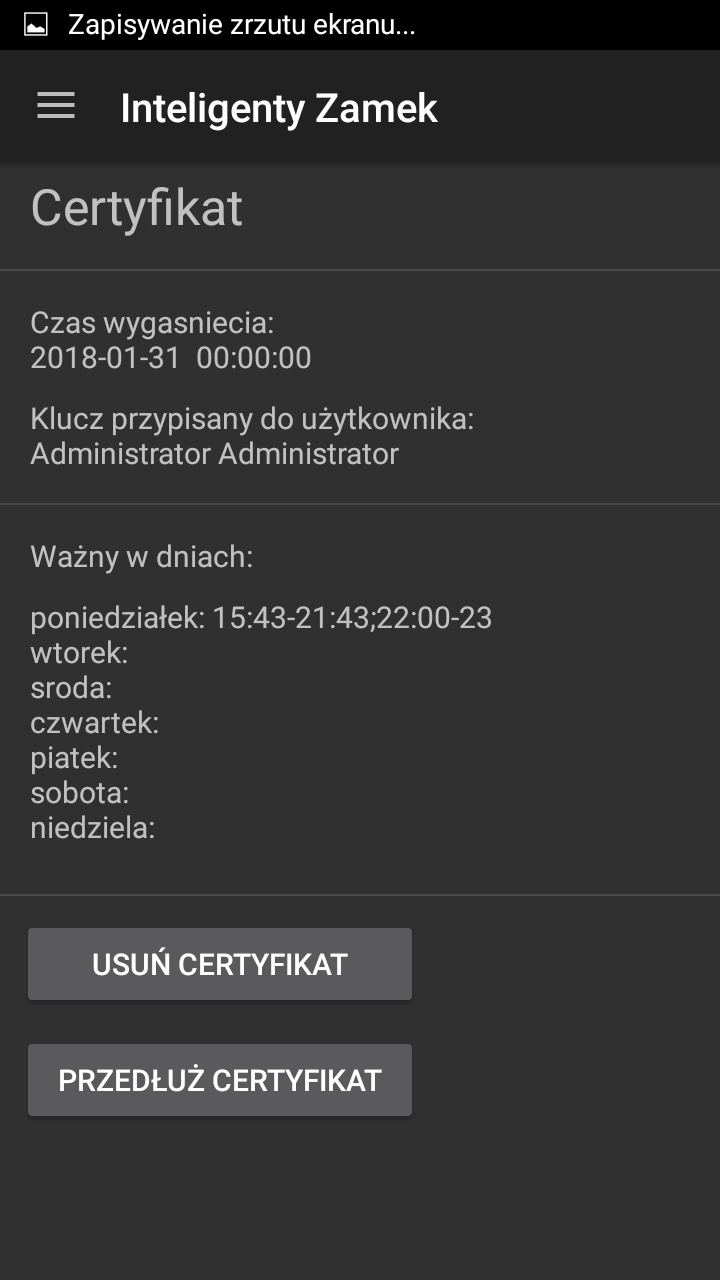
\includegraphics[width=\textwidth]{Obrazy/przedluzCert1}
			\caption{Stan początkowy listy oczekujących certyfikatów na zaakceptowanie }
			\label{rys:przedluzCert1}
		\end{minipage}
		
		\begin{minipage}{0.2\textwidth}
			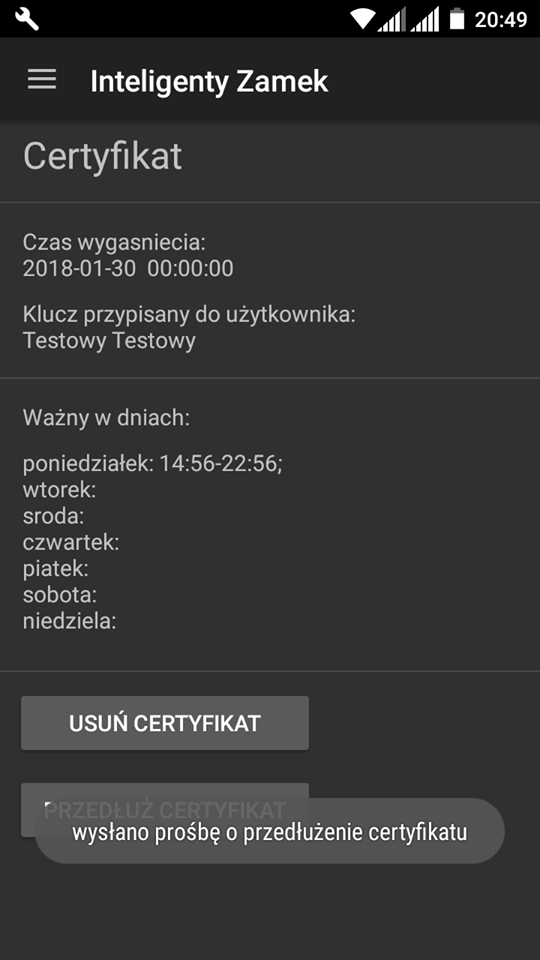
\includegraphics[width=\textwidth]{Obrazy/przedluzCert2}
			\caption{Stan początkowy listy oczekujących certyfikatów na zaakceptowanie }
			\label{rys:przedluzCert2}
		\end{minipage}
		
		
	
		
	\end{figure}
	
	
	\item M blokowanie certyfikatu szyfrującego *admin, user)
	\item M (admin) historia użycia zamka
	ukazanie historii zamka
	\item D zarządzanie kontami użytkowników
		Test polegał na wyświetleniu listy użytkowników zablokowaniu klucza dostępowego oraz konta.
		
		Wnioski: Podczas testu w stanie początkowym wszyscy użytkownicy systemu posiadali aktualny klucz dostępowy oraz nie byli zablokowani (Rys. \ref{rys:zarzadzanieKontem1}). Po zablokowaniu klucza dostępowego  Administratora zmienił się status na liście (Rys. \ref{rys:zarzadzanieKontem3}). Po Zablokowaniu konta użytkownika(Rys. \ref{rys:zarzadzanieKontem4}) również zmienił się status na liście (Rys. \ref{rys:zarzadzanieKontem5}). po wygenerowaniu ponownie klucza dostępowego nastąpiła zmiana statusu na liście (Rys. \ref{rys:zarzadzanieKontem6}). Próba zalogowania się na koncie zablokowanym nie doszła do skutku. Został wyświetlony komunikat ''Konto zostało zablokowane'' (Rys. \ref{rys:zarzadzanieKontem7}). Test przebiegł pomyślnie
		
		
				\begin{figure}[ht!]
					\begin{minipage}{0.2\textwidth}
						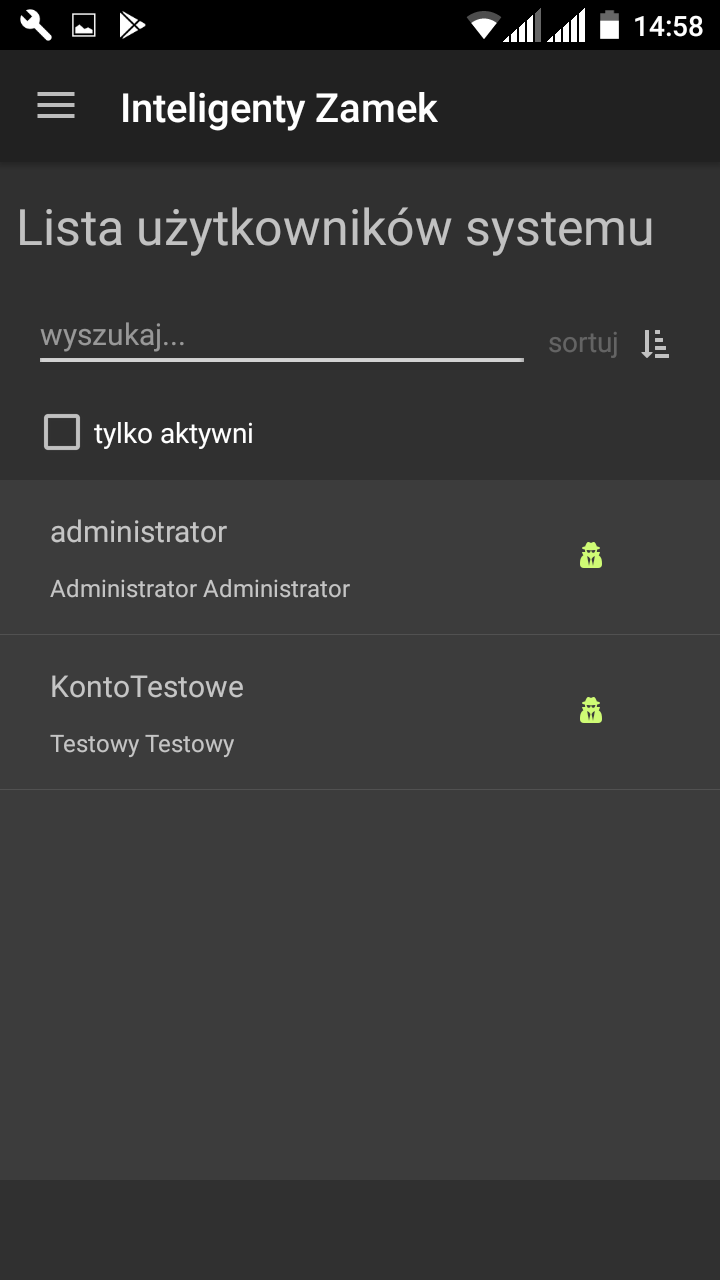
\includegraphics[width=\textwidth]{Obrazy/konto1}
						\caption{Stan początkowy listy oczekujących certyfikatów na zaakceptowanie }
						\label{rys:zarzadzanieKontem1}
					\end{minipage}
				\begin{minipage}{0.2\textwidth}
					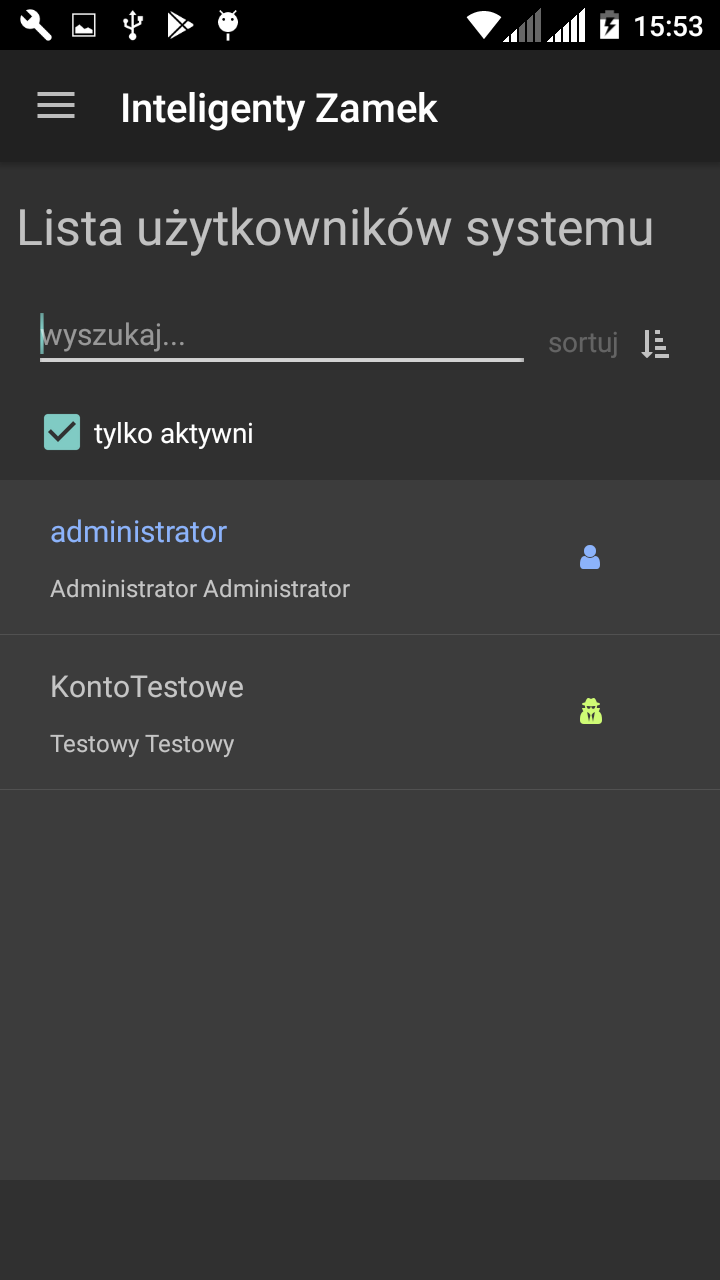
\includegraphics[width=\textwidth]{Obrazy/konto2}
					\caption{Stan początkowy listy oczekujących certyfikatów na zaakceptowanie }
					\label{rys:zarzadzanieKontem2}
				\end{minipage}
			
			\begin{minipage}{0.2\textwidth}
				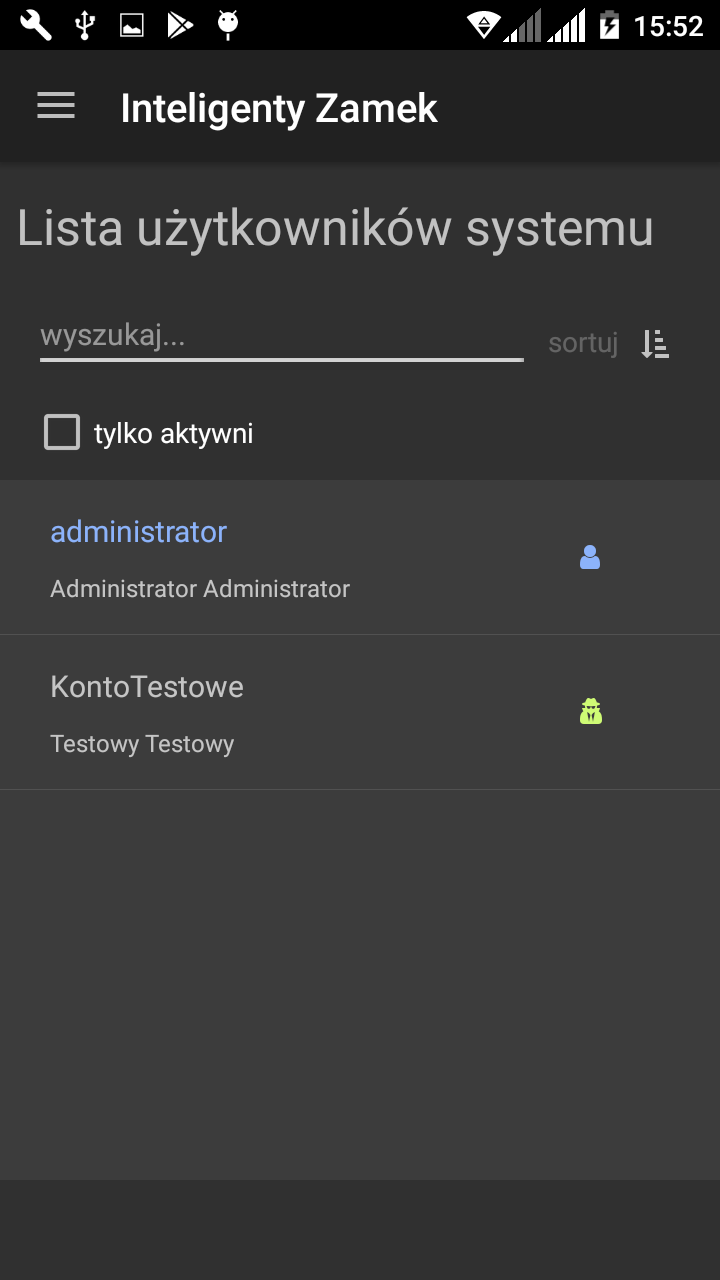
\includegraphics[width=\textwidth]{Obrazy/konto3}
				\caption{Stan początkowy listy oczekujących certyfikatów na zaakceptowanie }
				\label{rys:zarzadzanieKontem3}
			\end{minipage}
			
			\begin{minipage}{0.2\textwidth}
				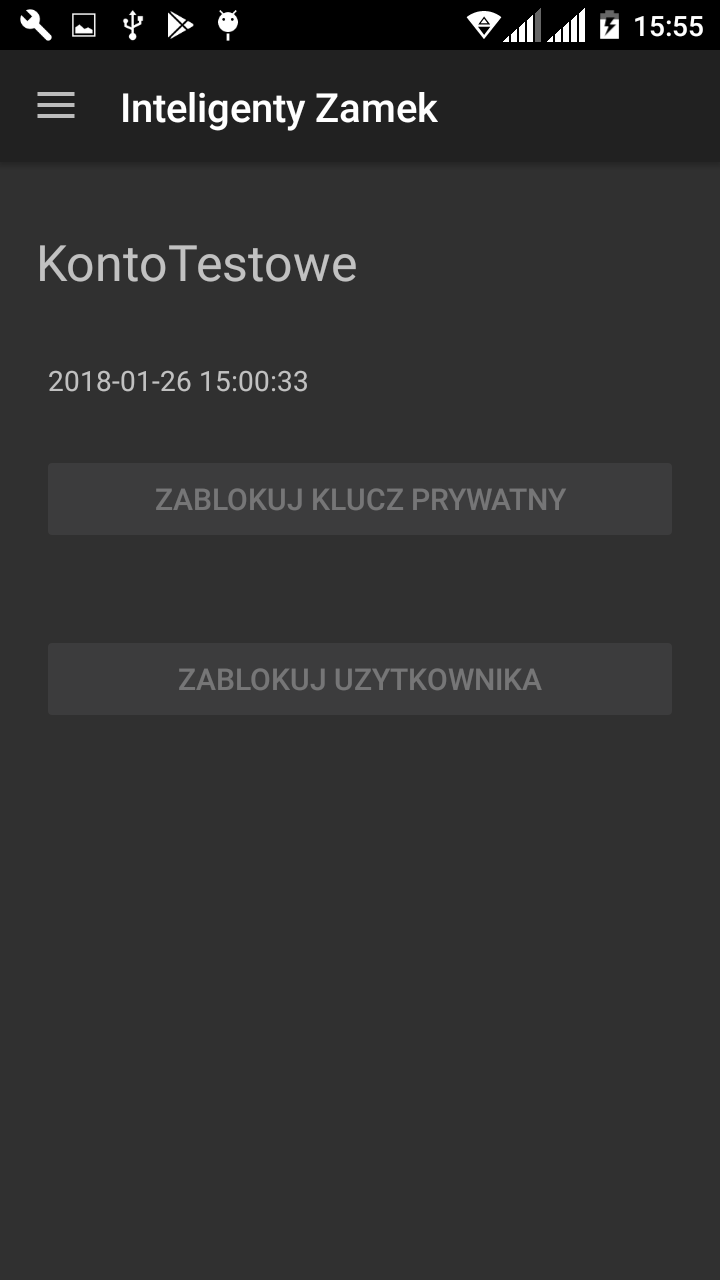
\includegraphics[width=\textwidth]{Obrazy/konto4}
				\caption{Stan początkowy listy oczekujących certyfikatów na zaakceptowanie }
				\label{rys:zarzadzanieKontem4}
			\end{minipage}
			
			
			\begin{minipage}{0.2\textwidth}
				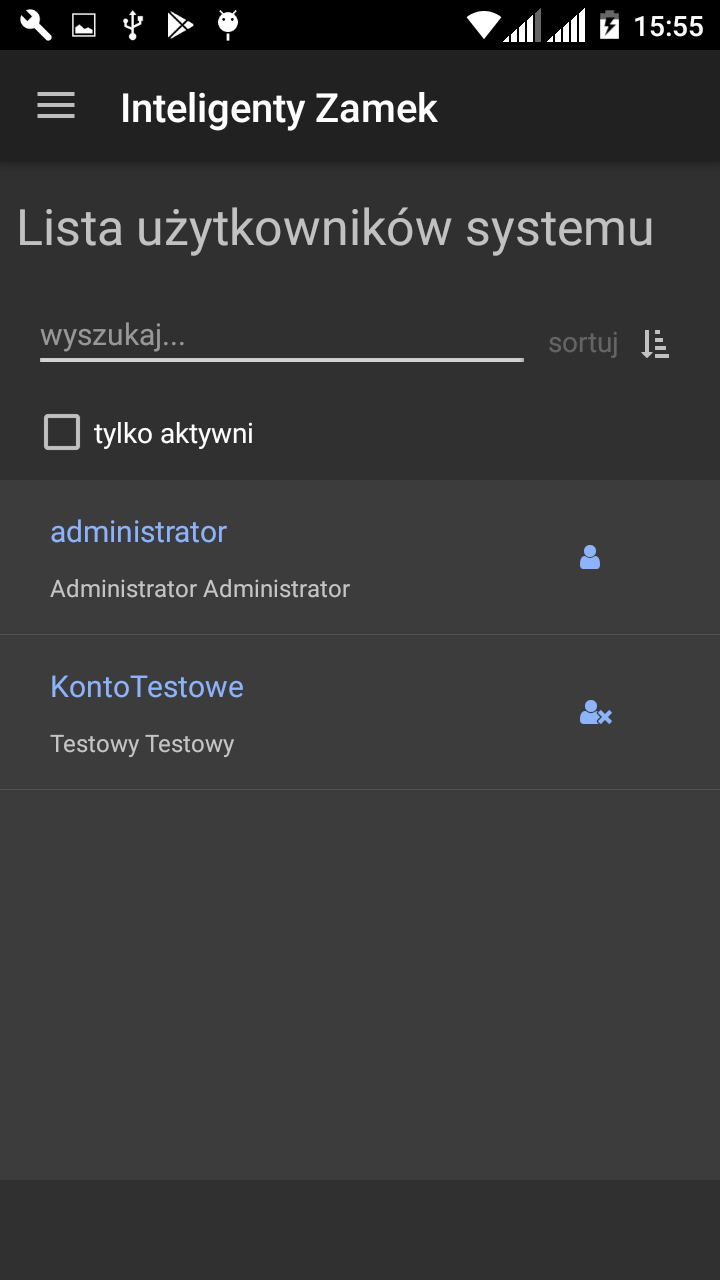
\includegraphics[width=\textwidth]{Obrazy/konto5}
				\caption{Stan początkowy podczas załadowania widoku wnioskowania o certyfikat}
				\label{rys:zarzadzanieKontem5}
			\end{minipage}
		
		
			\begin{minipage}{0.2\textwidth}
			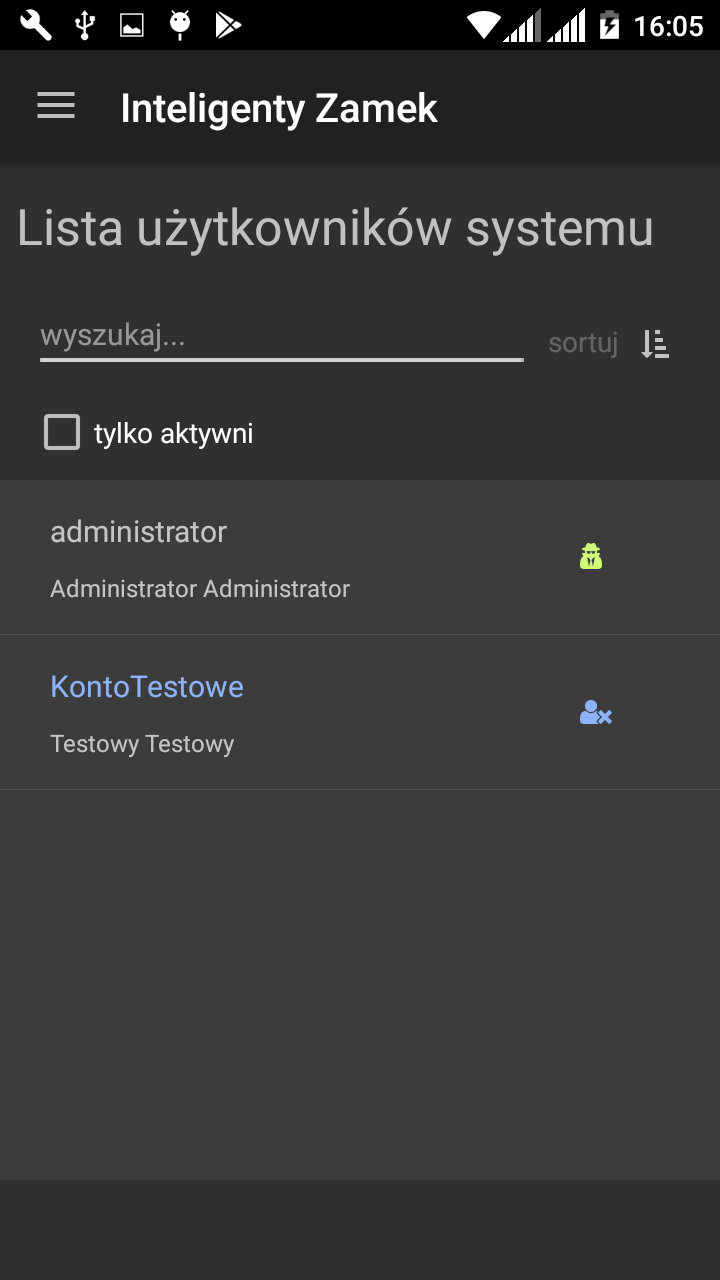
\includegraphics[width=\textwidth]{Obrazy/konto6}
			\caption{Stan początkowy podczas załadowania widoku wnioskowania o certyfikat}
			\label{rys:zarzadzanieKontem6}
		\end{minipage}
	
		\begin{minipage}{0.2\textwidth}
		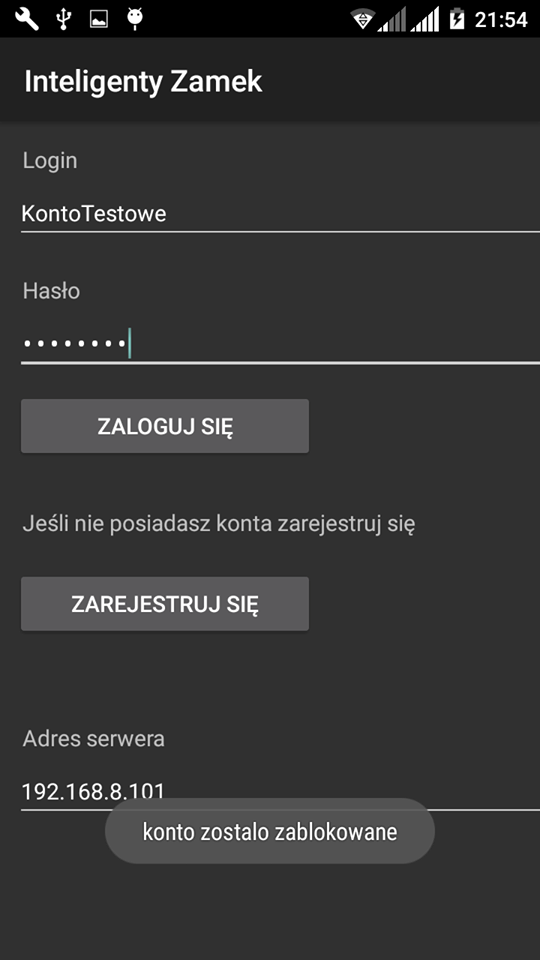
\includegraphics[width=\textwidth]{Obrazy/konto7}
		\caption{Stan początkowy podczas załadowania widoku wnioskowania o certyfikat}
		\label{rys:zarzadzanieKontem7}
	\end{minipage}

			
		\end{figure}
		
	\item  D eksport/import klucza
	Test polegał na eksporcie oraz imporcie klucza szyfrującego wraz z próbami niepoprawnego wpisywania hasła.
	
	Wnioski: Podczas próby eksportu z błędnie wprowadzonym hasłem została wyświetlona walidacja (Rys. \ref{rys:impExp1}) w postaci komunikatu ''niepoprawne hasło''. Po wprowadzeniu poprawnego hasła oraz eksporcie został wyświetlony komunikat (Rys. \ref{rys:impExp2} ''poprawnie wyeksportowano certyfikat''. Podczas próby importu z błędnie wprowadzonym hasłem został wyświetlony komunikat (Rys. \ref{rys:impExp1} ''niepoprawne hasło''. Po wprowadzeniu poprawnego hasła i ponownej próbie został wyświetlony komunikat (Rys. \ref{rys:impExp3} ''poprawnie zaimportowano certyfikat''. Test przebiegł pomyślnie.
	
	
	
	\begin{figure}[ht!]
		\begin{minipage}{0.2\textwidth}
			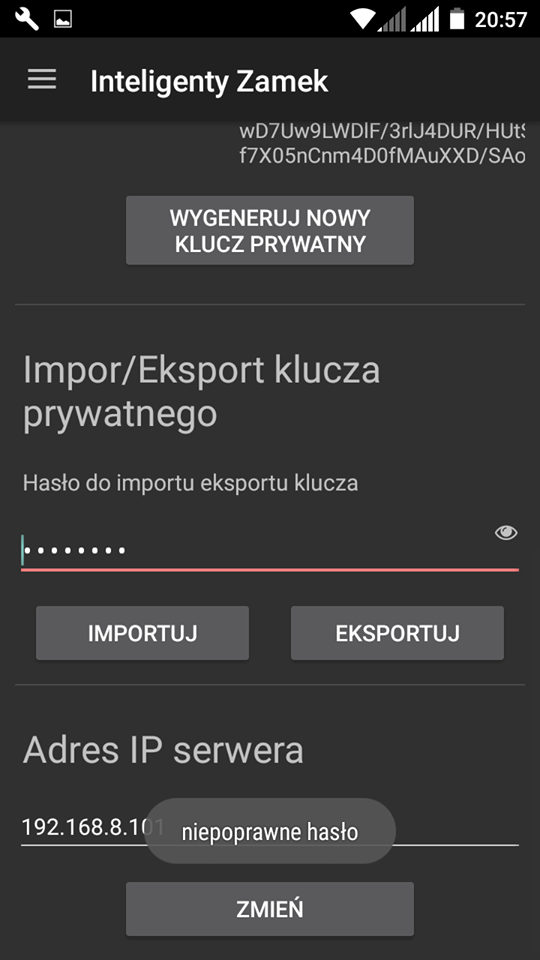
\includegraphics[width=\textwidth]{Obrazy/impExp1}
			\caption{Stan początkowy listy oczekujących certyfikatów na zaakceptowanie }
			\label{rys:impExp1}
		\end{minipage}
		\begin{minipage}{0.2\textwidth}
			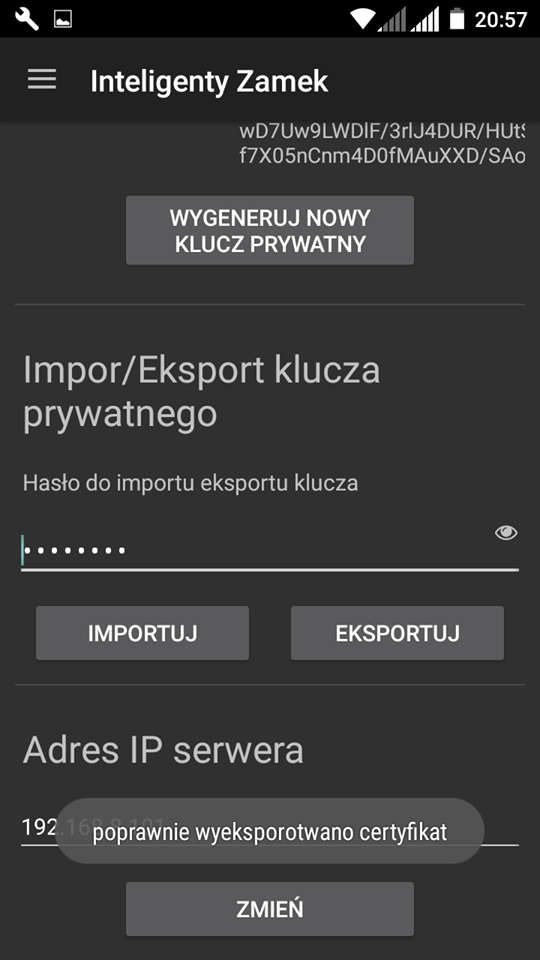
\includegraphics[width=\textwidth]{Obrazy/impExp2}
			\caption{Stan początkowy listy oczekujących certyfikatów na zaakceptowanie }
			\label{rys:impExp2}
		\end{minipage}
		
		\begin{minipage}{0.2\textwidth}
			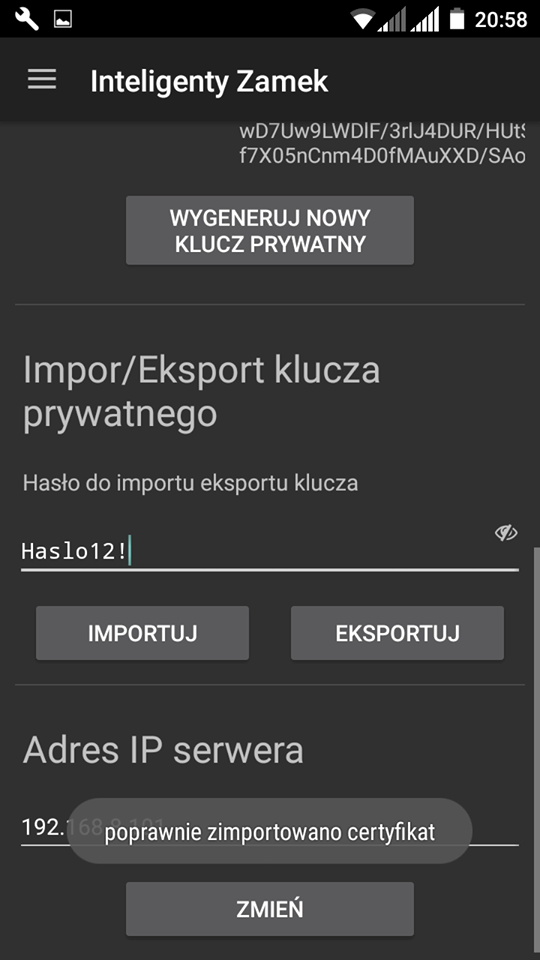
\includegraphics[width=\textwidth]{Obrazy/impExp3}
			\caption{Stan początkowy listy oczekujących certyfikatów na zaakceptowanie }
			\label{rys:impExp3}
		\end{minipage}
	\end{figure}
	
\end{enumerate*}
